\documentclass[12pt]{report}

\usepackage[T1]{fontenc}
\usepackage[utf8]{inputenc}
\usepackage{graphicx}

\begin{document}
{\Large \textbf{Drone.}\\}
\Large{Enesto Alonso Partida López\\ Universidad Politecnica De La Zona Metropolitana De Guadalajara\\ Mecatronica 4 A\\ Septiembre-diciembre 2019}\\
{18 de octubre 2019 }\\

\begin{center}

\includegraphics[scale=1]{../../../Downloads/upzmg.jpg} \\
\end{center}

\newpage
{\huge \textbf{DONIX.}}\\

{\huge \textbf{Planteamiento del problema.}}\\\\
{\large\textbf{ Existen ocaciones donde las personas que acampan el lugares alejados de la sociedad se extravian y para lograr localizarla pasa algunas horas debido a que la mayoria de la busqueda en por tierra o bien a pie, en muy pocas ocaciones se cuenta con un elicoptero, que ayude en la busqueda para posterior rescate, esto debido a lo costoso que es contratar a un piloto o el mismo elecoptero para la busqueda, por lo cual se pretende crear un pequeño drone que permita la busqueda por aire a una pequeña sona al rededor del piloto, lo cual incrementara la posibilidad de encontrar al o los extraviados.esto a la vez con un menor costo debido a que no se gasara en contratar un piloto y un elicoptero. mas sin embargo no se limitara en eso ya que se podra usar a la vez como un objeto para capturar tanto fotos como videos en caso de que el adquisitor lo desee.  }\\}


{\huge \textbf{Formular el problema}\\}\\
{\large \textbf{{debido al incremento de campistas en las zonas boscosas lo cual tambien incrementa laos extravios de personas por diversas situaciones, por lo cual su busqueda en ocaciones lleva hora o hasta dias, y a demas se tiene que recurrir tanto a equipo terrestre como aereo, por lo cual este apoyo aereo en ocaciones puede llagar a ser costoso, por lo cual se busca que cada rescatista cuante con un drone que pueda usar para buscar a su alrededor y asi poder localizar a el o los extraviados.  }}
\\\\


{\huge \textbf{Objetivo general del proyecto }\\}\\

{\large\textbf{ como a ido en aumento los extravios en zonas boscosas se pretende la creacion de un drone que permita a las autoridades la busqueda por aire con un menor costo y una eficiencia mayor, ya que como se ha dicho el contratar un elicoptero para la busqueda es muy costoso, por lo cual si cada rescatista opera un drone el area cubierta sera mayor por lo cual el localizar a los extraviados sera mas facil y en un menor tiempo.  }\\}

{\huge \textbf{Objetivo del proyecto  }\\}\\

{\large \textbf{ se realizara una investigacion previa para determinar si lo planteado es correcto y es necesario implementar un aparato para optimizar la busqueda de personas en zonas boscosas\\posterior mente se tendra que investigar que aparatos debera tener el drone para ayudar en la busqueda y ver si el personal esta capacitado o entiende la nocion de operar un drone.}\\}


\begin{table}[htb]
\centering
\begin{tabular}{| p{5.2cm}| p{10.2cm} |}
\hline
\multicolumn{2}{|c|}{Europa} \\
\hline
materia & objetivo \\
\hline \hline
Ingles & comprender la programacion del drone asi como el lenguaje de los materiales \\ \hline
Etica profesional & respetar el trabajo realizado por cada compañero. \\ \hline
Estructura y propiedad de los materiales & nos sera necesario para considerar los mejores materiales para la aelaboracion del drone \\ \hline
Programacion de perifericos & nos facilitara la programacion del drone en un lenguaje como c \\ \hline\\
Sistemas electronicos de interfaz & nos permitira controlar el torque y la velocidad del motor \\ \hline\\
Controladores logicos programables & controlar a larga distancia el drone asi como que cada motor se accione a su tiempo o cuando sea necesario \\ \hline\\
Habilidades generales & conocer los limites de cada compañero \\ \hline\\
Matematicas para ingenieria & nos facilitara conocer y entender cuales seran los mejores diseños para el chasis del drone asi como cuales podrian ser los mejores motores para dicho proyecto \\ \hline\\
Fisica para ingenieria & nos permitira darnos una idea de la estructura de algunos componentes asi como nos dara una mejor idea de que material usar para la fabricacion \\ \hline\\
Procesos  de manufactura & nos ayudra a planear el tiempo para la creacion del drone \\ \hline\\
Sistemas neumaticos e hidraulicos & nos permitira enfocarnos enel control del drone cuando este se encuentre volando \\ \hline\\
Liderazgo de equipos de alto desempeño & nos ayudara a repetar los horarios establecidos en el diagrama de gantt \\ \hline\\
Resistencia de materiales & nos permitira optar por un material resistente y durarero para el chasis del prototipo  \\ \hline
Cinematica de mecanismo & nos permitira hacer las comprovaciones y pruebas necesarias al drone \\ \hline 
Automatizacion industrial  & París \\ \hline
control de motores electricos   & nos permitira elegir los mejores motores para el prototipo a si como ver el funcionamiento y desgaste de los mismo  \\ \hline
\end{tabular}
\caption{Tabla de Relacion.}
\label{tabla:anchofijo}
\end{table}


{\huge \textbf{Justificacion }\\}


{\large\textbf{ debido a que sera una buena opcion para localizar personas en lugares de poco acceso a un bajo costo, a su vez como tendra un costo accesible el equipo de busqueda podra contar con mas de un drone para la localizacion del individuo.  }\\}



{\huge \textbf{Delimitacion }\\}


{\large \textbf{El drone tendra una dimencio superior a los 15 cm con un maximo de 50 cm, se espera que su peso sea menor a 2 kg para que sea faliz de trasportar, asi como, que cualquier persona sin experiencia previa pueda controlarlo, y sobretodo que si si el comprador decia pueda utilizarlo de otra manera segun sea su decicion. se preve que para finales del 6to cuatrimestre se entrege un prototipo semifuncional el cual se eleve del suelo unos pocos sentimetro por un corto periodo del tiempo, porque como se sabe crear algo de esta magnitud completamente funcional toma su tiempo, cabe de resaltar que el prototipo solo tendra una pila con poca duracion ya que es una prueba del diseño} }\\ \\


\begin{table}[htb]
\centering
\begin{tabular}{| p{2.2cm}| p{2.2cm} |}
\hline
\multicolumn{2}{|c|}{Europa} \\
\hline
Material & Costo \\
\hline \hline
Motores BRUSHLESS & 600 \\ \hline
Aspas & 300 \\ \hline
Controlador de vuelo & 1200 \\ \hline
Reseptor & 300 \\ \hline
Modulo led & 120 \\ \hline
Bateria de litio & 350 \\ \hline
Chasis & 700 \\ \hline
\end{tabular}
\caption{Tabla de Materiales.}
\label{tabla:anchofijo}
\end{table}
\begin{table}[htb]
\centering
\begin{tabular}{| p{2.2cm}| p{4.2cm} |}
\hline
\multicolumn{2}{|c|}{Europa} \\
\hline
integrante & tarea \\
\hline \hline
Alosno & Cotizar los materiales, Optener los materiales, Armado del prototipo, Relizar los reportes e invertigacion, Conseguir patrocinio para que el gasto sea menor \\ \hline

\end{tabular}
\caption{Tabla de Roles.}
\label{tabla:anchofijo}
\end{table}
\begin{table}[htb]
\centering
\begin{tabular}{| p{3.2cm}| p{4.2cm} |}
\hline
\multicolumn{2}{|c|}{Europa} \\
\hline
Materias de 4to & Aportacion  \\
\hline \hline
ingles & comprender el lenguaje de programacion \\ \hline
Etica profesional & valorar el trabajo realizado asi como tener una satisfaccion por realizarlo  \\ \hline
Estructura y propiedad de los materiales & conocer cual es el mejor material para que el drone sea lijero y funcione correctamente \\ \hline
Programacion de perifericos & sera necesario una programacion la cual nos servira para controlar el drone\\ \hline
Sistemas electronicos de interfaz & el control de los motores para delimitar que tan rapido o lento deben jirar\\ \hline
Controladores logicos programables & el armado del circuito interno del drone \\ \hline

\end{tabular}
\caption{Tabla de Relacion con Materias de 4to.}
\label{tabla:anchofijo}
\end{table}
\newpage
{\Large Daigrama de GANTT}\\
\begin{figure}[hbtp]
\caption{Diagrama de GANTT}
\centering
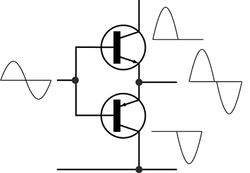
\includegraphics[scale=0.4]{../../1.png}
\end{figure}


\end{document}